
\chapter{平台软件规划——连接确认(CC)}

 参考文件: Module Design of XX (Template).xlsx \cite{MDOT1};   
  
 \begin{enumerate}[label=\textbullet]
	\item  Introduce;
        \begin{enumerate}[label={}]
            \item \textcolor{red}{A brief description of the design module, which explains the functions that the modules needs to implement;}
        \end{enumerate}
	\item  Module Ports;
        \begin{enumerate}[label={}]
            \item \textcolor{red}{Don't need to write the specific ports, just write ``For more details about the modules ports, please refer to the related module interface files";}
        \end{enumerate}
	\item  Design Contents;
        \begin{enumerate}[label={}]
            \item \textcolor{red}{Before starting the design, the engineer should read the relevant information in ReadMe;}
        \end{enumerate}
\end{enumerate}

PP(Proximity Pilot)功能:PP 信号主要用于检测充电枪的物理状态,即充电插头的插
入深度和连接情况。PP 信号通过在插头和插座之间的物理连接来检测接近状态。作用:确认
充电枪是否插入到位。防止在插头未完全插入的情况下启动充电。确定充电电缆的额定电流
上限,以便限制通过充电线缆的最大电流,避免电缆过载。

CC(Connection Confirmation)功能:CC 信号负责最终确认连接的整体安全性,并在
充电开始前完成所有必要的检查。它通常依赖于 CP 和 PP 信号提供的信息,以确定是否可以
安全地开始充电。作用:确认 PP 信号的接近检测状态,以及 CP 信号的通信和控制状态。在
确认连接安全、无误后,允许充电电流传输。如果在充电过程中发现任何异常情况,CC 信号
将触发充电中断。

本文档适用于充电设备在{\bf 充电模式2 连接方式B}工作状态下的使用规范。

\section{Introduce}
 连接确认模块(Connect comfirm),在SAE\_J1772中是接近检测(Proximity Detection)\cite{SAE}。 
 这两个信号的关系不一致: PP $\longrightarrow$ CP $\longrightarrow$ CC。

 PP信号主要用于检测充电枪的物理状态,即充电插头的插入深度和连接情况。PP信号通过在插头和插座之间的物理连接来检测接近状态。
 \begin{enumerate}
    \item  确认充电枪是否插入到位;
    \item  防止在插头未完全插入的情况下启动充电;
    \item  确定充电电缆的额定电流上限,以便限制通过充电线缆的最大电流,避免电缆过载。
 \end{enumerate}

 \begin{figure}[!htbp]
    \centering
    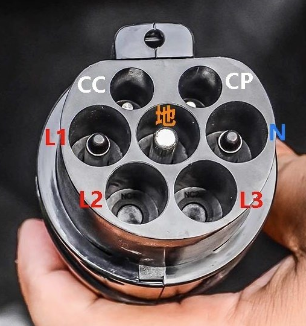
\includegraphics[width = 0.45\textwidth]{C3}
    \caption{交流充电接口}
    \label{fig:C3}
\end{figure}

\begin{figure}[!htbp]
    \centering
    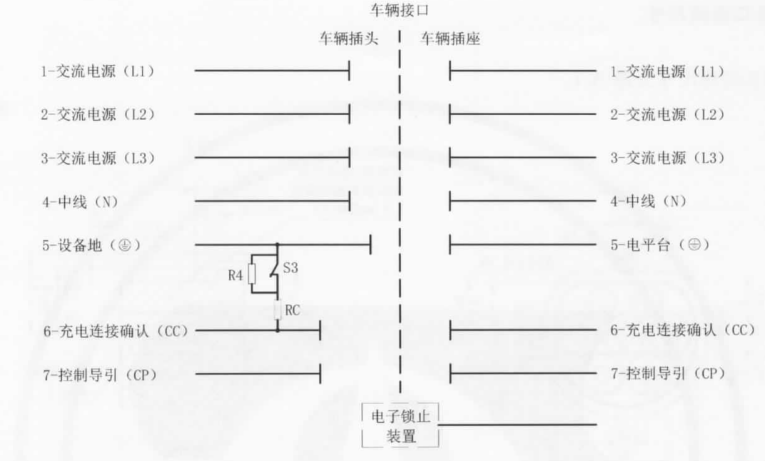
\includegraphics[width = 0.65\textwidth]{C5}
    \caption{车辆接口电气连接示意图}
    \label{fig:C5}
\end{figure}

\section{Modules Ports}


\section{Design Contents}

(1) 车辆控制装置测量检测点 2 有无 12 V CP 信号。如有
则标志着车辆插头与车辆插座已连接,控制导引电
路激活进入工作状态;如无,则控制导引电路处于
待机状态。%[8]。

(2) 车辆控制装置通过测量检测点 3 与
PE 之间的电阻值来判断车辆插头与车辆插座是否
完全连接。半连接时,S3 断开,检测点 3 与 PE 之
间的电阻为 RC+R4;完全连接时,S3 处于闭合状
态,检测点 3 与 PE 之间的电阻值为 RC。

(3) 供电控制装置通过测量检测点 1 的电压判断 R3 是否接
入,如 R3 接入则延时一定时间,将 S1 切换至 PWM输出状态。

(4) 车辆检测装置通过测量检测点 2 的
PWM 信号,判断充电装置是否已经完全连接。如
完全连接,则闭合开关 S2,车辆进入准备就绪状态。

(5) 供电控制装置通过进一步测量检测点 1 的电压
判断车辆是否进入准备就绪状态,如已进入就绪状
态,则闭合 K1、K2,交流供电回路导通。%[11]。

(6) 车辆控制装置通过测量检测点 2 的 PWM 信号占空比
确认供电设备的最大供电能力,并以此确定车载充
电机的输出电流,启动充电过程。%[9]。


\begin{figure}[!htbp]
    \centering
    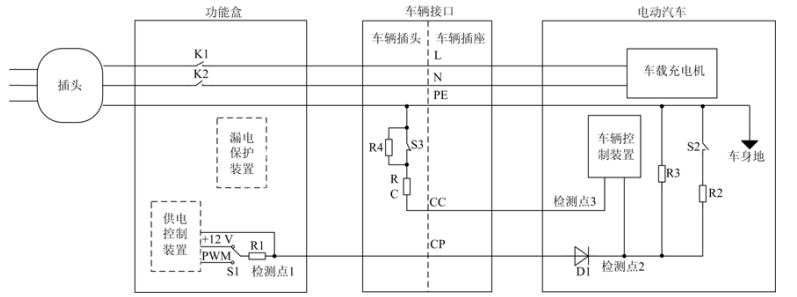
\includegraphics[width = 0.72\textwidth]{C4}
    \caption{交流充电模式2连接方式B}
    \label{fig:C3}
\end{figure}